% !TEX program = xelatex
\documentclass[a4paper,14pt,oneside,openany]{memoir}

%%% Задаем поля, отступы и межстрочный интервал %%%

\usepackage[left=30mm, right=15mm, top=20mm, bottom=20mm]{geometry}
\pagestyle{plain}
\parindent=1.25cm
\usepackage{indentfirst}

%%% Задаем языковые параметры и шрифт %%%

\usepackage[english,russian]{babel}
\babelfont[russian]{rm}{Times New Roman}
\babelfont[russian]{tt}{Courier New}

%%% Задаем стиль заголовков и подзаголовков в тексте %%%

\setsecnumdepth{subsection}
\renewcommand*{\chapterheadstart}{}
\renewcommand*{\printchaptername}{}
\renewcommand*{\chapnumfont}{\normalfont\bfseries}
\renewcommand*{\afterchapternum}{\hspace{1em}}
\renewcommand*{\printchaptertitle}{\normalfont\bfseries\centering\MakeUppercase}
\setbeforesecskip{20pt}
\setaftersecskip{20pt}
\setsecheadstyle{\raggedright\normalfont\bfseries}
\setbeforesubsecskip{20pt}
\setaftersubsecskip{20pt}
\setsubsecheadstyle{\raggedright\normalfont\bfseries}

%%% Исправление нумерации секций %%%

\renewcommand{\thesection}{\arabic{section}}
\renewcommand{\thesubsection}{\arabic{subsection}}

%%% Сквозная нумерация рисунков и таблиц %%%

\counterwithout{figure}{chapter}
\counterwithout{table}{chapter}

%%% Выравнивание и переносы %%%

\tolerance 1414
\hbadness 1414
\emergencystretch 1.5em
\clubpenalty=10000
\widowpenalty=10000

%%% Задаем параметры оформления рисунков и таблиц %%%

\usepackage{graphicx}
\usepackage{caption}
\usepackage{subcaption}
\usepackage{float}
\graphicspath{{photo/}}
\captionsetup[figure]{font=small, width=\textwidth, name=Рисунок, justification=centering}
\captiondelim{ --- }
\usepackage[section]{placeins}

%%% Задаем параметры ссылок и гиперссылок %%% 

\usepackage{hyperref}
\hypersetup{
    colorlinks=true,
    linkcolor=red,
    citecolor=red
}

%%% Настраиваем отображение списков %%%

\usepackage{enumitem}
\renewcommand*{\labelitemi}{\normalfont{--}}
\setlist{noitemsep, leftmargin=*}

\begin{document}

% Титульный лист (без номера страницы)
\thispagestyle{empty}

\begin{center}
    МИНИСТЕРСТВО ЦИФРОВОГО РАЗВИТИЯ, СВЯЗИ И МАССОВЫХ \\ КОММУНИКАЦИЙ \\ РОССИЙСКОЙ ФЕДЕРАЦИИ

    \vspace{20pt}

    Федеральное государственное бюджетное образовательное учреждение \\ высшего образования \\
    "Сибирский государственный университет телекоммуникаций и \\ информатики"

    \vspace{20pt}

    Кафедра телекоммуникационных систем и вычислительных средств \\ (ТС и ВС)
\end{center}

\vfill

\begin{center}
    Практическая работа №6 \\
    по дисциплине \\
    \textit{"Web-технологии"}

    \vspace{20pt}

    по теме: \\
    \uppercase{Облачное файловое хранилище Seafile}
\end{center}

\vfill

\noindent Студент: \\
\textit{Группа ИКС-532 \hfill А.С. Лёшин}

\vspace{20pt}

\noindent Преподаватель: \\
\textit{старший преподаватель \hfill А.В. Андреев}

\vfill

\begin{center}
    Новосибирск 2026 г.
\end{center}

\newpage
\setcounter{page}{2}
\OnehalfSpacing*

\subsection*{Цель работы}
\begin{itemize}
    \item Развернуть облачное файловое хранилище Seafile на отдельной виртуальной машине;
    \item Настроить сетевые параметры и DNS-записи для доступа к серверу;
    \item Выполнить установку и настройку Seafile с использованием MariaDB в качестве базы данных;
    \item Проверить работоспособность системы через веб-интерфейс.
\end{itemize}

\section{Подготовка инфраструктуры}

Первым этапом настройки является присвоение серверу корректного имени. На \hyperref[fig:rename]{рисунке \ref*{fig:rename}} показан процесс переименования виртуального сервера в seafile.

\begin{figure}[H]
    \centering
    
\includegraphics[width=0.6\textwidth]{photo/photo3.png}
    \caption{Переименование виртуального сервера в seafile}
    \label{fig:rename}
\end{figure}

Далее выполняется настройка статического IP-адреса в файле \texttt{/etc/netplan/00-installer-config.yaml}. На \hyperref[fig:static_IP]{рисунке \ref*{fig:static_IP}} представлено содержимое данного файла после редактирования.

\begin{figure}[H]
    \centering
    
\includegraphics[width=0.6\textwidth]{photo/photo1.png}
    \caption{Содержимое файла /etc/netplan/00-installer-config.yaml}
    \label{fig:static_IP}
\end{figure}

Проверить правильность настройки можно командой \texttt{ip a}. На \hyperref[fig:ipa]{рисунке \ref*{fig:ipa}} представлен вывод команды.

\begin{figure}[H]
    \centering
    
\includegraphics[width=0.6\textwidth]{photo/1.png}
    \caption{Вывод команды ip a}
    \label{fig:ipa}
\end{figure}

Также проверяется доступность внешних ресурсов командой \texttt{ping ya.ru}. На \hyperref[fig:ya]{рисунке \ref*{fig:ya}} показан результат.

\begin{figure}[H]
    \centering
    
\includegraphics[width=0.6\textwidth]{photo/photo2.png}
    \caption{Вывод команды ping ya.ru}
    \label{fig:ya}
\end{figure}

\section{Настройка DNS}

Для корректной работы сервера необходимо добавить прямую и обратную записи в DNS на сервере Gateway. На \hyperref[fig:forward]{рисунке \ref*{fig:forward}} показан процесс добавления прямой записи в домен, а на \hyperref[fig:reverse]{рисунке \ref*{fig:reverse}} — обратной записи.

\begin{figure}[H]
    \centering
    
\includegraphics[width=0.8\textwidth]{photo/photo4.png}
    \caption{Добавление прямой записи в DNS}
    \label{fig:forward}
\end{figure}

\begin{figure}[H]
    \centering
    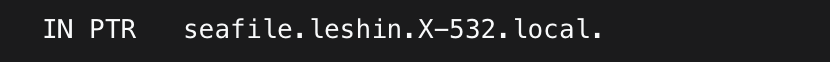
\includegraphics[width=0.8\textwidth]{photo/photo4.2.png}
    \caption{Добавление обратной записи в DNS}
    \label{fig:reverse}
\end{figure}

После добавления записей выполняется проверка работоспособности DNS. На \hyperref[fig:DNS]{рисунке \ref*{fig:DNS}} представлен результат запроса.

\begin{figure}[H]
    \centering
    
\includegraphics[width=0.8\textwidth]{photo/photo5.png}
    \caption{Проверка работы DNS}
    \label{fig:DNS}
\end{figure}

\section{Установка и настройка Seafile}

\subsection{Установка пакетов и зависимостей}

Были установлены необходимые системные пакеты, MariaDB и Python-зависимости. Установка Seafile выполнена с использованием официального дистрибутива для архитектуры ARM64.

\subsection{Попытка запуска и возникшие проблемы}

При попытке запуска веб-интерфейса командой \texttt{./seahub.sh start} возникли ошибки, связанные с несовместимостью версий Python и библиотек.

На \hyperref[fig:configuration]{рисунке \ref*{fig:configuration}} представлен вывод завершения установки Seafile.

\begin{figure}[H]
    \centering
    
\includegraphics[width=0.8\textwidth]{photo/photo6.png}
    \caption{Завершение установки Seafile}
    \label{fig:configuration}
\end{figure}

На \hyperref[fig:error1]{рисунке \ref*{fig:error1}} представлена ошибка, возникшая при попытке запуска \texttt{seahub.sh}.

\begin{figure}[H]
    \centering
    
\includegraphics[width=0.8\textwidth]{photo/photo7.png}
    \caption{Ошибка AttributeError: module 'pkgutil' has no attribute 'ImpImporter'}
    \label{fig:error1}
\end{figure}

В процессе устранения ошибок были предприняты следующие действия:

\begin{enumerate}
    \item Установлены недостающие системные библиотеки (\texttt{libffi-dev}, \texttt{libtiff5-dev});
    \item Выполнена замена устаревших вызовов \texttt{ANTIALIAS} на \texttt{LANCZOS} в файлах конфигурации;
    \item Создана программная заглушка для замены \texttt{MySQLdb} на \texttt{pymysql};
    \item Синхронизированы версии библиотеки \texttt{cffi} в каталоге Seafile и системе;
    \item Предпринята попытка развертывания через Docker-контейнер.
\end{enumerate}

\subsection{Дополнительные попытки устранения проблемы}

После неудачного запуска Seafile на виртуальной машине под управлением VirtualBox были предприняты дополнительные попытки развертывания системы в альтернативных средах:

\begin{enumerate}
    \item \textbf{Попытка установки в UTM.} Была предпринята попытка развернуть Seafile в программе UTM, оптимизированной для работы на процессорах Apple Silicon. Установка выполнялась с использованием тех же дистрибутивов и по той же методике. Результат оказался идентичным — ошибка \texttt{AttributeError: module 'pkgutil' has no attribute 'ImpImporter'} возникала на том же этапе запуска \texttt{seahub.sh}.

    \item \textbf{Использование различных версий Ubuntu.} Для проверки совместимости были протестированы следующие версии операционной системы:
    \begin{itemize}
        \item Ubuntu 22.04 LTS (Jammy Jellyfish) — установка выполнена полностью, однако ошибка при запуске Seafile сохранилась;
        \item Ubuntu 22.04 с дополнительными репозиториями Python — попытка установить Python 3.10 параллельно с системным не привела к успеху.
    \end{itemize}

    \item \textbf{Смена архитектуры и версий Seafile.} В процессе отладки использовались различные дистрибутивы Seafile:
    \begin{itemize}
        \item Seafile 9.0.9 для ARM64 (основная попытка);
        \item Seafile 10.0.1 для ARM64 — установка прошла, но ошибка с \texttt{pkgutil} осталась;
        \item Docker-образ seafileltd/seafile-mc:latest — контейнер запустился, но MySQL внутри не инициализировался.
    \end{itemize}

        \item \textbf{Ручная корректировка кода.} В ходе отладки вручную исправлялись следующие участки кода:
    \begin{itemize}
        \item Замена \texttt{ImpImporter} на \texttt{zipimporter} в файле \texttt{pkg\_resources/init.py};
        \item Замена \texttt{ANTIALIAS} на \texttt{LANCZOS} в \texttt{avatar/settings.py};
        \item Создание символической ссылки \texttt{Image} на \texttt{PIL} в каталоге thirdpart;
        \item Установка и подмена \texttt{MySQLdb} на \texttt{pymysql}.
    \end{itemize}
\end{enumerate}

Все перечисленные попытки не привели к успешному запуску Seafile. Проблема носит системный характер и связана с несовместимостью кодовой базы Seafile 9.x с Python 3.12 и архитектурой ARM64.

\section{Выявленные проблемы}

Основные причины, препятствующие успешному запуску Seafile:

\begin{enumerate}
    \item \textbf{Несовместимость с Python 3.12.} Seafile 9.0.9 разработан для Python 3.8–3.10, в то время как на используемой системе установлен Python 3.12.
    \item \textbf{Отсутствие поддержки ARM64 в некоторых библиотеках.} Часть зависимостей не имеет готовых сборок для архитектуры ARM64.
    \item \textbf{Устаревшие API в новых версиях библиотек.} Pillow 12.x использует \texttt{LANCZOS} вместо устаревшего \texttt{ANTIALIAS}, что вызывает ошибки в коде Seafile.
    \item \textbf{Изменения в стандартной библиотеке Python 3.12.} Удаление атрибута \texttt{ImpImporter} из модуля \texttt{pkgutil} нарушает работу некоторых компонентов Seafile.
    \item \textbf{Системный характер проблемы.} Ошибка воспроизводится на разных гипервизорах (VirtualBox, UTM), на разных версиях Ubuntu (22.04, 24.04) и с разными версиями Seafile (9.0.9, 10.0.1). Это указывает на фундаментальную несовместимость Seafile с современными версиями Python на ARM-архитектуре.
\end{enumerate}

\section*{Заключение}
\addcontentsline{toc}{section}{Заключение}

В ходе выполнения работы были выполнены следующие задачи:

\begin{enumerate}
    \item Подготовлена инфраструктура — создана ВМ seafile с статическим IP-адресом 192.168.14.4;
    \item Настроены DNS-записи для корректного разрешения имени seafile.leshin.X-532.local;
    \item Установлены MariaDB и необходимые Python-пакеты;
    \item Произведена установка Seafile с использованием официального дистрибутива для ARM64;
    \item Выполнен анализ ошибок, возникающих при запуске, и предприняты попытки их устранения;
    \item Проведены дополнительные тесты в альтернативных средах (UTM, разные версии Ubuntu, разные версии Seafile).
\end{enumerate}

Запустить Seafile на используемой платформе (Ubuntu 24.04 ARM64, Python 3.12) не удалось ввиду несовместимости версий. Все подготовительные этапы были выполнены успешно, что подтверждает корректность настройки сетевой и DNS-инфраструктуры.

\end{document}